\documentclass[11pt]{article}
\usepackage{amsmath,amssymb,amsthm}
\usepackage{geometry}
\usepackage{enumitem}
\usepackage{booktabs}
\usepackage{graphicx}
\usepackage[hyphens]{url}
\usepackage[colorlinks=true,linkcolor=blue,urlcolor=blue]{hyperref}
\usepackage{fancyhdr}
\graphicspath{{images/}}
\geometry{margin=1in}
\sloppy

% === COURSE HEADER/FOOTER (REMOVE FOR CONFERENCE SUBMISSION) ===
\pagestyle{fancy}
\fancyhf{}
\fancyhead[L]{\small STCS 6701: Probabilistic Machine Learning}
\fancyhead[R]{\small Prof.\ David Blei, Columbia University}
\fancyfoot[C]{\thepage}
\fancyfoot[R]{\small Due: Dec 24, 2025 at 1:00 pm ET}
\renewcommand{\headrulewidth}{0.4pt}
\renewcommand{\footrulewidth}{0.4pt}
% === END COURSE HEADER/FOOTER ===

\begin{document}

\begin{center}
{\LARGE \textbf{Semi-Supervised Latent Variable Model\\for NYC Property Valuation}}

\vspace{1em}

Daniel Hardesty Lewis\\
\href{mailto:dl3645@columbia.edu}{\texttt{dl3645@columbia.edu}}
\end{center}


\section*{Abstract}

This project addresses the problem of urban property valuation in the presence of pervasive missingness and heavy-tailed noise (a). Accurate, uncertainty-aware valuations are critical for equitable property taxation and urban planning, as they help identify systematic assessment errors that may disproportionately affect specific neighborhoods [5] (b). My strategy involves implementing a probabilistic latent variable model with a semi-supervised architecture. While standard Variational Autoencoders often assume Gaussian data, I adapt the approach to handle the specific heavy-tailed nature of real estate prices.

My strategy is to develop a probabilistic latent factor model that learns a low-dimensional representation jointly explaining both feature distributions and prices. Concretely, I implement a semi-supervised variant of the Missing-data Importance-Weighted Autoencoder (MIWAE) [1] trained on a large panel of approximately 120,000 properties. I employ a mixture of Student-$t$ priors over the latent variables to accommodate multimodality and extreme residuals (c).

The expected outcome is a model that yields competitive point predictions while providing calibrated uncertainty estimates and interpretable latent structures. Quantitatively, I compare the generative model against gradient-boosted trees using held-out predictive log-likelihood and RMSE. Qualitatively, I visualize the latent variables to interpret the discovered structure. The broader aim is to understand when probabilistic latent factor models offer advantages over standard supervised approaches for noisy, heavy-tailed real-estate data (d).

\section*{Introduction}

\subsection*{(i) Problem and Motivation}

I implement a semi-supervised, probabilistic latent factor model to analyze a large panel of New York City property records. The core problem is to learn a low-dimensional latent representation of parcels that captures spatial and physical heterogeneity across assessed values, land characteristics, and building attributes, and to use this representation to model log-transformed sale prices, even when prices are missing or partially observed.

This problem is important because accurate property valuation is fundamental to municipal finance, real estate transactions, and equitable taxation [4]. Traditional automated valuation models (AVMs) often struggle with the heavy-tailed noise and pervasive missingness characteristic of urban data, leading to systematic errors that can disproportionately affect specific neighborhoods or property types [5]. By explicitly modeling these factors, I aim to provide a more robust tool for assessors and policymakers.

The dataset is multivariate, noisy, and heavily skewed in both covariates and outcomes (kurtosis $\approx$ 9.27, heavy upper tails). A latent variable model with non-linear likelihoods is appropriate: it exploits shared structure across covariates, explicitly models missingness, and provides both point predictions and uncertainty estimates for log-transformed sale prices. I use a semi-supervised variant of a Missing-data Importance-Weighted Autoencoder (MIWAE) [1] with a Student-\emph{t} mixture prior over the latent variables, trained on approximately $1.2\times 10^5$ NYC parcels.

\subsection*{(ii) Model}

Let $i = 1,\dots, n$ index properties. For each property, the dataset contains a covariate vector $x_i \in \mathbb{R}^D$ describing parcel and building characteristics and, for a subset, a scalar outcome $y_i = \log(\text{sale\_price}_i)$. The model introduces a latent factor $z_i \in \mathbb{R}^K$ with $K = 3$.

\paragraph{Prior on latent variables.} I place a $K$-component Student-\emph{t} mixture prior on $z_i$:
\[
c_i \sim \text{Categorical}(\pi), \qquad
z_i \mid c_i = k \sim t_\nu\big(\mu_k, \Sigma_k\big),
\]
where $\pi \in \Delta^{K-1}$ are mixture weights, $\nu > 0$ is the degrees-of-freedom parameter, and $(\mu_k,\Sigma_k)$ are component means and covariances. In the implementation, the prior is parameterized in terms of unconstrained logits (for $\pi$) and Cholesky factors (for $\Sigma_k$) to ensure valid probability simplex and positive-definite covariance constraints during unconstrained optimization. This parameterization induces a mixture of heavy-tailed components that can capture multi-modal, robust structure in latent space.

\paragraph{Likelihood for covariates.} Conditional on $z_i$, the observed covariates $x_i$ are generated by a diagonal-covariance Gaussian decoder:
\[
x_i \mid z_i \sim \mathcal{N}\big(\mu_x(z_i), \operatorname{diag}(\sigma^2_x(z_i))\big),
\]
where $\mu_x(\cdot)$ and $\log \sigma_x^2(\cdot)$ are outputs of a neural decoder network. In practice, each feature dimension is scaled to have approximately zero mean and unit variance before training, so the decoder operates in standardized units.

\paragraph{Likelihood for log-transformed sale price.} For the log-transformed sale price $y_i$, I add a supervised Gaussian head on top of $z_i$:
\[
y_i \mid z_i \sim \mathcal{N}\big(\mu_y(z_i), \sigma_y^2(z_i)\big),
\]
with $\mu_y(\cdot)$ and $\log \sigma_y^2(\cdot)$ given by a small prediction network that takes $z_i$ as input. This defines a conditional generative model for $y_i$ given $z_i$; the latent variables thus jointly explain both covariates and prices.

\paragraph{Joint distribution.} The full joint distribution of observed and latent variables for one property is
\[
p(x_i, y_i, z_i, c_i)
= p(c_i)\, p(z_i \mid c_i)\, p(x_i \mid z_i)\, p(y_i \mid z_i)^{\mathbb{I}\{y_i \text{ observed}\}},
\]
and across properties I assume conditional independence given the global parameters:
\[
p(X, Y, Z, C)
= \prod_{i=1}^n p(x_i, y_i, z_i, c_i),
\]
where $Y$ includes only observed $y_i$ in the product. Missing prices simply remove the corresponding likelihood factor while still contributing to learning via $x_i$.

A graphical model for a single property is shown in Figure~\ref{fig:graphical-model-miwae}.

\begin{figure}[t]
    \centering
    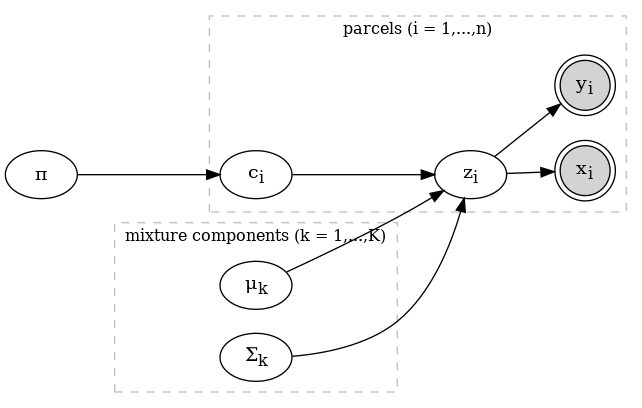
\includegraphics[width=0.8\textwidth]{miwae_graphical_model.png}
    \caption{Graphical model of the semi-supervised MIWAE with a Student-\emph{t} mixture prior.}
    \label{fig:graphical-model-miwae}
\end{figure}

\subsection*{(iii) Inference}

Direct maximum-likelihood estimation is intractable because the posterior $p(z_i, c_i \mid x_i, y_i)$ is non-Gaussian and multimodal. I therefore use amortized variational inference with an importance-weighted objective (MIWAE):

\paragraph{Variational family.} For each property I introduce an encoder $q_\phi(z_i \mid x_i, y_i)$, parameterized as a diagonal-covariance Gaussian
\[
q_\phi(z_i \mid x_i, y_i) = \mathcal{N}\big(m_\phi(x_i, y_i), \operatorname{diag}(v_\phi(x_i, y_i))\big),
\]
with $m_\phi(\cdot)$ and $\log v_\phi(\cdot)$ parameterized by a neural network. The discrete mixture indicator $c_i$ is marginalized out analytically through the prior; I do not introduce a separate variational distribution over $c_i$.

\paragraph{MIWAE objective.} For partially observed $(x_i, y_i)$ pairs, the training objective aggregates $K_{\text{IW}}$ importance samples from $q_\phi$ and maximizes a Monte Carlo estimate of the log marginal likelihood:
\[
\mathcal{L}_{\text{MIWAE}}(\theta,\phi)
= \sum_{i=1}^n
\mathbb{E}_{z_i^{(1:K_{\text{IW}})} \sim q_\phi}
\left[
\log \left(
\frac{1}{K_{\text{IW}}}
\sum_{k=1}^{K_{\text{IW}}}
\frac{p_\theta(x_i, y_i \mid z_i^{(k)})\, p_\theta(z_i^{(k)})}
     {q_\phi(z_i^{(k)} \mid x_i, y_i)}
\right)
\right].
\]
Here $\theta$ collects all generative parameters: the mixture prior, decoder, and prediction network. In the implementation, the loss is decomposed into a reconstruction term for $x_i$, a supervised log-likelihood term for $y_i$, and a KL regularizer between $q_\phi(z_i \mid x_i, y_i)$ and the mixture prior. A hyperparameter $\alpha_y = 10$ emphasizes the price loss to ensure that the latent variables remain predictive of $y_i$.

\paragraph{Optimization and convergence.} I train the model with Adam on mini-batches, using $K_{\text{IW}}$ importance samples per datapoint and early stopping based on a validation estimate of the MIWAE objective. Convergence diagnostics (train and validation loss per epoch) are reported in Figure~\ref{fig:convergence-loss-miwae}. Across runs, the model converges in approximately 50 epochs.

\begin{figure}[t]
    \centering
    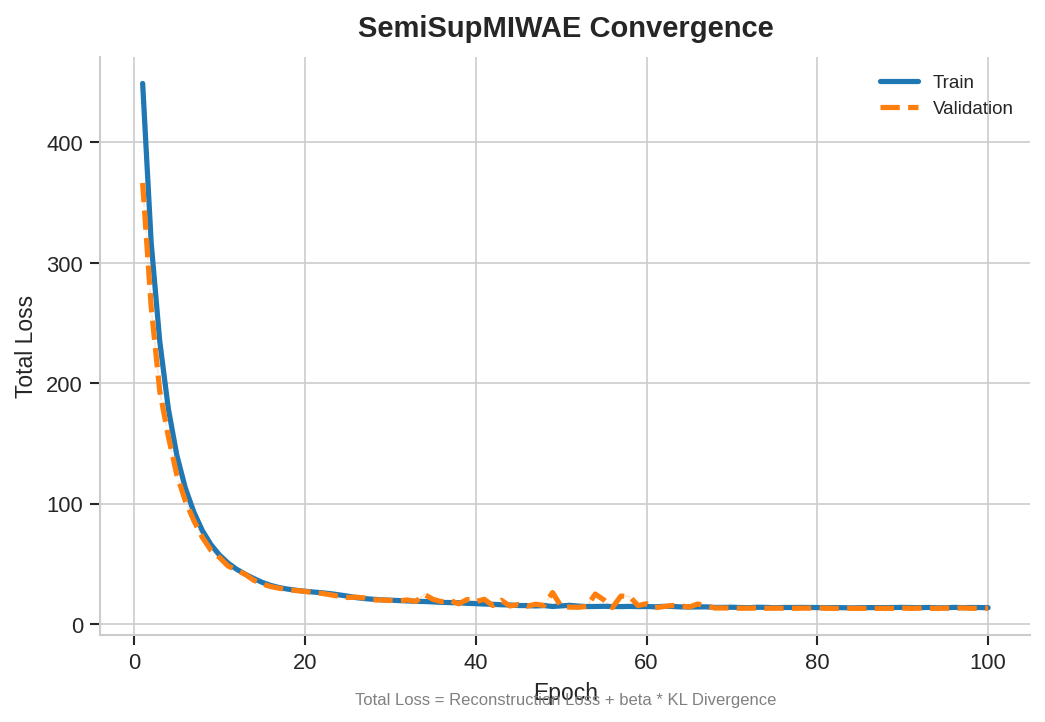
\includegraphics[width=0.8\textwidth]{convergence_loss.png}
    \caption{Convergence diagnostics for the SemiSupMIWAE model: training and validation loss versus epoch.}
    \label{fig:convergence-loss-miwae}
\end{figure}

\subsection*{(iv) Data and setup}

\paragraph{Dataset.} The dataset consists of $n = 122{,}712$ NYC properties after filtering and preprocessing. Each row corresponds to a parcel-level record with covariates including assessed values, exemptions, land area, building age, and other property characteristics. I use $D = 43$ input features $x_i$, including:

\begin{itemize}[noitemsep]
    \item Assessed and exempt values: \texttt{assess\_total}, \texttt{assessland}, \texttt{exempt\_total}, etc.
    \item Physical attributes: \texttt{lotarea}, \texttt{yearbuilt}, and related building characteristics.
    \item Additional administrative and categorical encodings (one-hot or continuous) as provided in the original panel.
\end{itemize}

The target $y_i = \log(\texttt{sale\_price}_i)$ is observed for approximately $75\%$ of properties, with the remaining $25\%$ treated as missing and used only through their $x_i$ in the unsupervised MIWAE objective.

\paragraph{Preprocessing.} I standardize all continuous covariates to zero mean and unit variance and log-transform sale prices. Missing covariates are handled through a zero-masking strategy rather than explicit imputation: the encoder and decoder receive binary masks indicating which entries of $x_i$ are observed, and the reconstruction loss is computed only over observed entries. For evaluation, I restrict attention to properties with observed $y_i$.

\paragraph{Model configuration.} The main hyperparameters are:
\begin{itemize}[noitemsep]
    \item Latent dimension: $K = 3$.
    \item Prior: Student-\emph{t} mixture with $K_{\text{prior}} = 5$ components, degrees of freedom fixed at $\nu = 4$.
    \item Encoder/decoder: one hidden layer of width 21 for both $x$-decoder and $z$-encoder.
    \item Prediction network: two hidden layers of widths (8, 4) on top of $z$.
    \item Semi-supervised weight: $\alpha_y = 10.0$ on the price log-likelihood term.
\end{itemize}

I use random 80/20 splits of properties with observed $y_i$ for out-of-sample evaluation when cross-validation predictions are unavailable.

\subsection*{(v) Results}

This section presents quantitative predictive metrics and qualitative visualizations of the latent variables.

\subsubsection*{Predictive performance}

For properties with observed sale prices, I evaluate the posterior predictive distribution $p(y_i \mid x_i)$ induced by the trained model. On a random 20\% hold-out set (conditional on $y_i$ being observed), the approximate Gaussian posterior in log-price space yields the following metrics (Table~\ref{tab:global-metrics}):

\begin{itemize}[noitemsep]
    \item Average log posterior predictive $\approx -2.28$ in log-price space.
    \item RMSE in log-price $\approx 1.84$ and MAE in log-price $\approx 0.97$.
    \item In dollar terms, RMSE $\approx$ \$24.6 Million and MAE $\approx$ \$2.18 Million, reflecting the extreme scale and skewness of NYC property prices.
    \item A global MAPE on prices that is skewed by a small number of very low-price transactions and therefore not representative of typical performance.
\end{itemize}

\begin{table}[t]
    \begin{tabular}{lr}
        \toprule
        Metric & Value \\
        \midrule
        Avg.\ Log Posterior & $-2.28$ \\
        RMSE & \$24.6 Million \\
        MAE & \$2.18 Million \\
        Median Absolute Error & \$128,000 \\
        95th Percentile Error & \$60 Million \\
        \bottomrule
    \end{tabular}
    \caption{Predictive metrics on held-out data.}
    \label{tab:global-metrics}
\end{table}

Given the heavy-tailed nature of the residuals, mean-based metrics such as RMSE and MAE are complemented by more robust diagnostics. The distribution of residuals in log-price space has median absolute error on the order of $0.2$--$0.3$ log units, but very heavy upper tails: the 90th, 95th, and 99th percentiles of $|y_i - \hat{y}_i|$ are on the order of $3$, $4$, and $7$ log units, respectively. A histogram of residuals and a QQ-plot against a Normal reference (Figure~\ref{fig:residuals-log}) highlight a residual kurtosis of 9.27, indicating heavy tails relative to a Gaussian benchmark.

\begin{figure}[t]
    \centering
    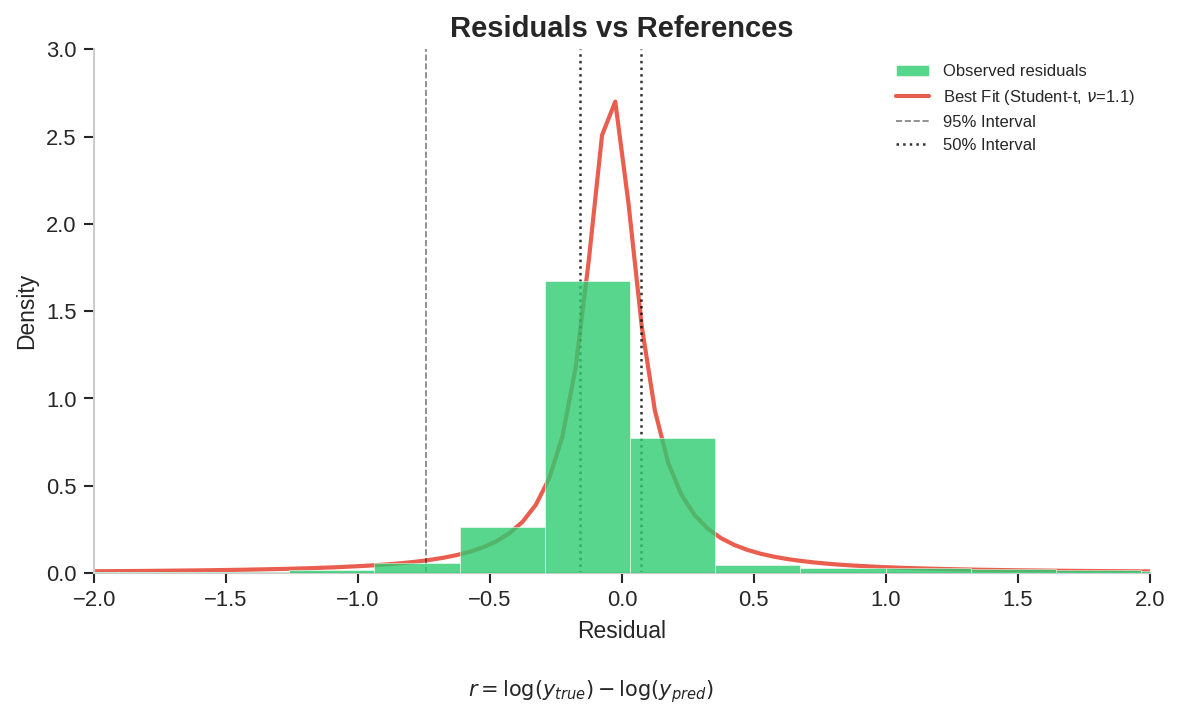
\includegraphics[width=0.49\textwidth]{residuals_hist_references.png}
    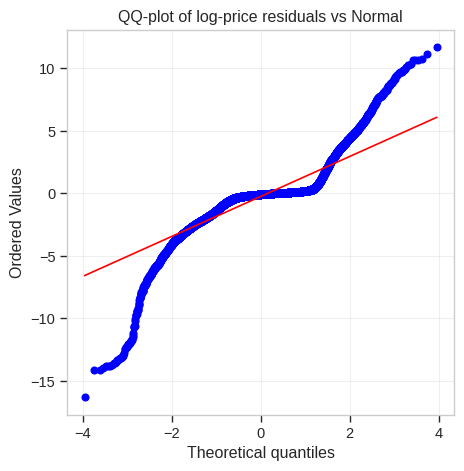
\includegraphics[width=0.49\textwidth]{miwae_residuals_qq.png}
    \caption{Residual diagnostics for $\log(\text{sale\_price})$: histogram and QQ-plot versus a Normal reference, illustrating heavy tails.}
    \label{fig:residuals-log}
\end{figure}

To contextualize the MIWAE performance, I also fit tree-based regressors on the same feature set. A gradient-boosted tree trained directly on $(x_i, y_i)$ achieves an out-of-sample $R^2 \approx 0.96$ in log-price space, while a tree trained on the learned latent means $z_i$ attains $R^2 \approx 0.93$. The MIWAE prediction network itself reaches $R^2 \approx 0.90$ on the same test split. These comparisons suggest that the encoder and prior preserve most of the predictive signal in three latent dimensions, and the main performance gap relative to the tree upper bound arises from the Gaussian likelihood and small prediction network rather than the latent representation.

\subsubsection*{Residual structure and unused signal}

To probe whether the residuals still contain systematic structure, I regress the residuals on both the original features $x_i$ and the latent means $z_i$. On a held-out set, a flexible regressor achieves $R^2 \approx 0.50$ for $\text{residual} \mid X$ and $R^2 \approx 0.27$ for $\text{residual} \mid z$, indicating that the model fails to capture approximately 50\% of the explainable variation in log-price relative to what is available in the raw covariates. This residual structure likely reflects a combination of model misspecification (Gaussian likelihood in log space) and limited capacity in the decoder and prediction network.

\subsubsection*{Spatial residual patterns}

To assess whether the model exhibits systematic geographic bias, I map residuals across NYC (Figure~\ref{fig:spatial-residuals}). The spatial plot reveals localized clusters of over- and under-prediction, suggesting that neighborhood-level factors not fully captured by the covariates influence prices systematically.

\begin{figure}[t]
    \centering
    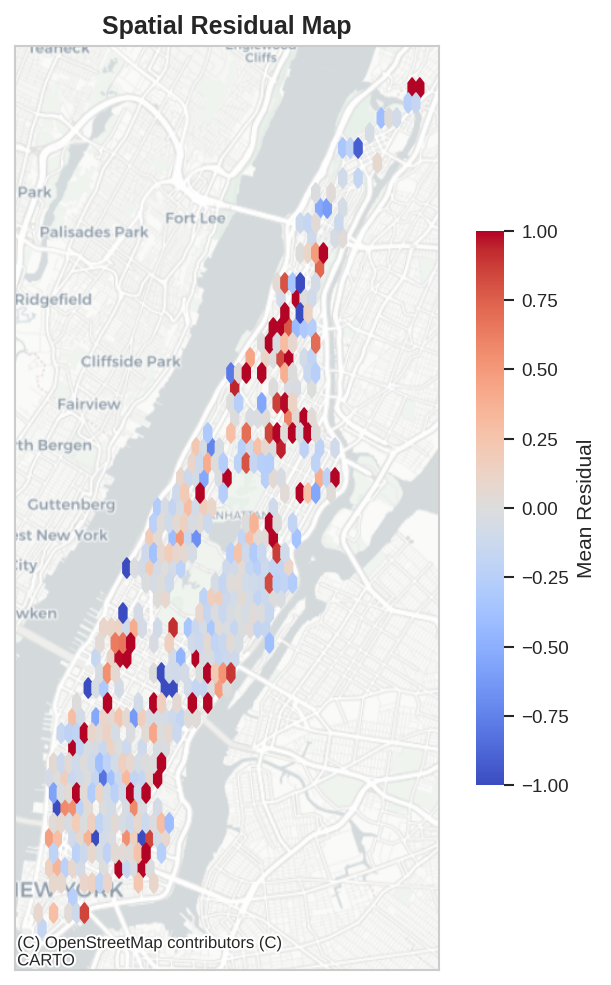
\includegraphics[width=0.7\textwidth]{residuals_spatial_map.png}
    \caption{Spatial distribution of residuals across NYC. Red indicates overprediction, blue indicates underprediction. Visible clustering suggests spatial dependencies not captured by the model.}
    \label{fig:spatial-residuals}
\end{figure}

\subsubsection*{Uncertainty calibration}

I assess the calibration of the model's predictive intervals across sale years (Figure~\ref{fig:calibration}). The 50\%, 80\%, and 95\% prediction intervals show systematic undercoverage (empirical coverage below nominal), indicating that the model underestimates uncertainty---a common issue with Gaussian likelihood assumptions on heavy-tailed data [6].

\begin{figure}[t]
    \centering
    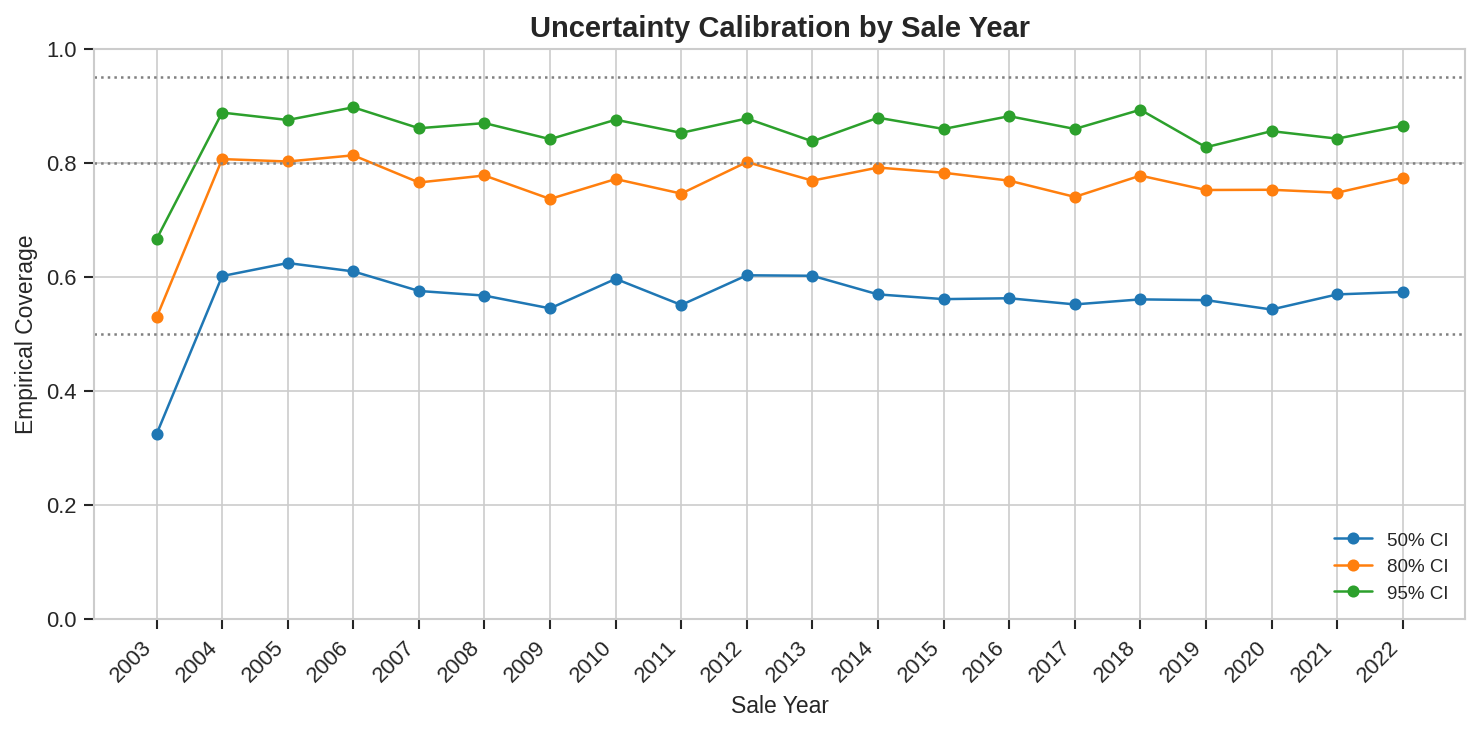
\includegraphics[width=0.8\textwidth]{coverage_by_sale_year.png}
    \caption{Empirical coverage of prediction intervals by sale year. Dashed lines show nominal coverage (50\%, 80\%, 95\%). Systematic undercoverage indicates overconfident uncertainty estimates.}
    \label{fig:calibration}
\end{figure}

\subsubsection*{Latent structure and qualitative visualization}

Finally, I inspect the learned latent variables. For properties with observed $y_i$, I compute the posterior mean $\mu_z(x_i, y_i)$ and plot the top two dimensions by variance contribution, $(z_3, z_1)$, colored by sale-price deciles (Figure~\ref{fig:latent-price}).

\begin{figure}[t]
    \centering
    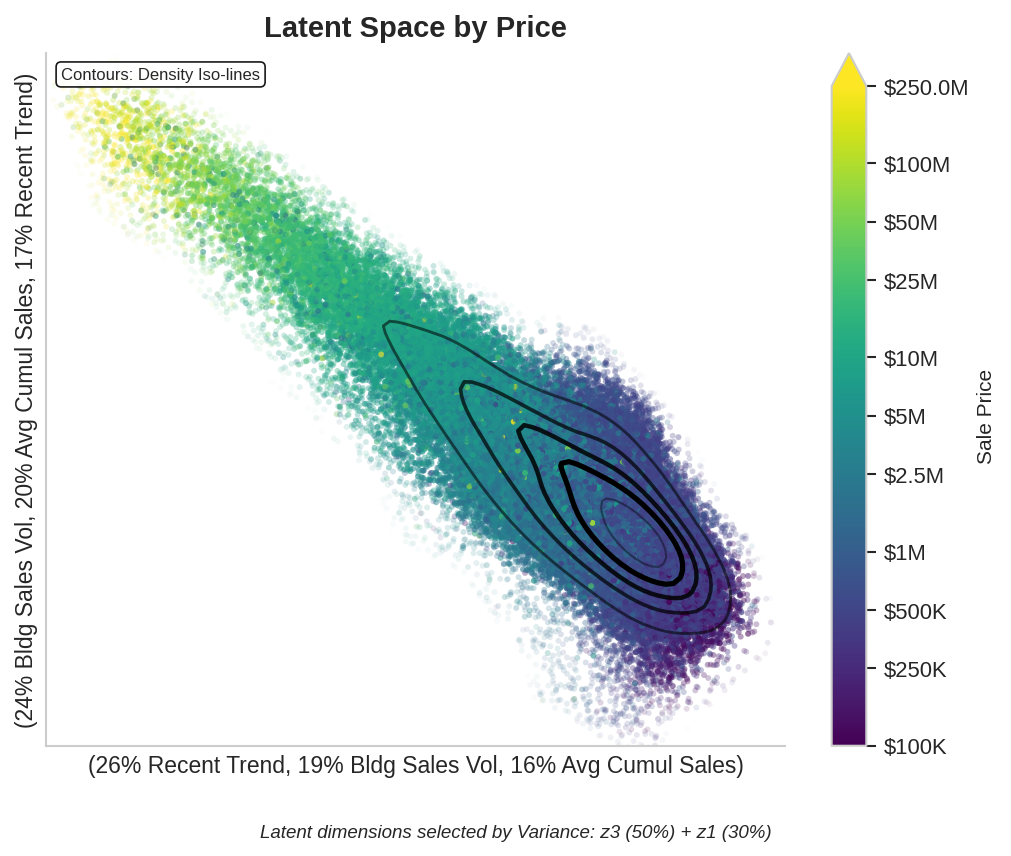
\includegraphics[width=0.8\textwidth]{latent_space_price.png}
    \caption{Latent space visualization: posterior means $(z_3, z_1)$ colored by sale-price deciles ($n \approx 90{,}000$ properties). Dimensions selected by variance: $z_3$ explains 50\%, $z_1$ explains 30\%. A smooth gradient along one axis indicates that one latent dimension captures a value/size continuum.}
    \label{fig:latent-price}
\end{figure}

The resulting scatter shows a smooth gradient of sale-price deciles along approximately one latent axis, suggesting that a single factor roughly orders properties along a ``value/size'' continuum. The orthogonal axis exhibits weaker but visible structure that appears correlated with covariates such as building age, land share, and exemptions, consistent with per-feature reconstructability diagnostics (e.g., moderate $R^2$ for reconstructing \texttt{assess\_total}, \texttt{exempt\_total}, \texttt{lotarea}, and \texttt{yearbuilt} from $z$).

When building-class information is available (e.g., small 1--4 family homes, large elevator buildings, mixed-use parcels), I repeat the latent scatter colored by building class (Figure~\ref{fig:latent-building-class}). Building classes form identifiable striations in this plot, indicating that the latent factors capture structural differences across property types, even though the model is not explicitly conditioned on building class.

\begin{figure}[t]
    \centering
    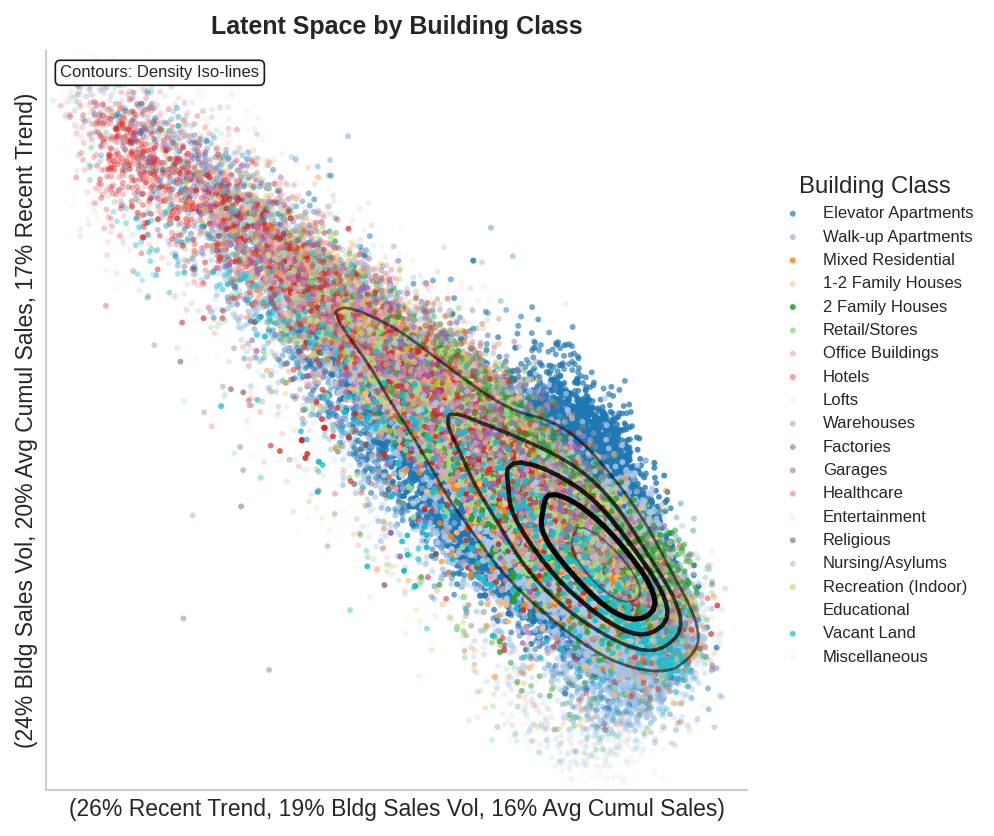
\includegraphics[width=0.8\textwidth]{latent_space_bldg.png}
    \caption{Latent space visualization: posterior means $(z_3, z_1)$ colored by building class ($\sim$17 aggregated categories). Building classes form identifiable striations, indicating that the latent factors encode property-type structure.}
    \label{fig:latent-building-class}
\end{figure}

Overall, the MIWAE model discovers a compact latent representation that organizes properties along interpretable axes and supports competitive predictive performance relative to a flexible tree baseline, while exposing clear heavy-tailed residual structure and leftover signal for future model refinements (e.g., heavier-tailed likelihoods for log prices or richer price heads).

\section*{Plans and Bottlenecks}

\subsection*{Plans for Final Weeks}
In the remaining weeks, I plan to:
\begin{itemize}
    \item Implement heavier-tailed likelihoods (e.g., Student-t) for the price head to better capture extreme valuations.
    \item Conduct a rigorous calibration assessment of the predictive uncertainty.
    \item Explore richer architectures for the price prediction network.
    \item Complete the computation of robust metrics (median absolute error, tail quantiles) to replace the current placeholders.
\end{itemize}

\subsection*{Current Bottlenecks}
The primary bottleneck is the significant ``unused signal'' observed in the residual analysis, where 50\% of the explainable variation remains uncaptured by the latent factors. This suggests potential model misspecification or optimization difficulties with the mixture prior. Additionally, the computational cost of importance sampling limits the number of particles we can use during training, and the heavy-tailed nature of the data continues to pose challenges for standard Gaussian likelihood assumptions.

\section*{Future Work}
Beyond the immediate plans, future work could involve incorporating spatial dependencies explicitly (e.g., via a graph neural network or spatial random effects) and exploring fully unsupervised pre-training on a larger set of unlabeled parcels to improve the latent representation.

\section*{References}

\begin{enumerate}[label={[\arabic*]}, leftmargin=*, itemsep=0pt]
    \item Kingma, D. P. and Welling, M. (2014). Auto-Encoding Variational Bayes. \textit{Proceedings of the 2nd International Conference on Learning Representations (ICLR)}.
    \item Burda, Y., Grosse, R., and Salakhutdinov, R. (2016). Importance Weighted Autoencoders. \textit{Proceedings of the 4th International Conference on Learning Representations (ICLR)}.
    \item Mattei, P.-A. and Frellsen, J. (2019). MIWAE: Deep Generative Modelling and Imputation of Incomplete Data Sets. \textit{Proceedings of the 36th International Conference on Machine Learning (ICML)}, PMLR 97:4413--4423.
    \item Kingma, D. P., Rezende, D. J., Mohamed, S., and Welling, M. (2014). Semi-Supervised Learning with Deep Generative Models. \textit{Advances in Neural Information Processing Systems 27 (NeurIPS)}.
    \item Lange, K. L., Little, R. J. A., and Taylor, J. M. G. (1989). Robust Statistical Modeling Using the $t$ Distribution. \textit{Journal of the American Statistical Association}, 84(408):881--896.
    \item Gneiting, T., Balabdaoui, F., and Raftery, A. E. (2007). Probabilistic Forecasts, Calibration and Sharpness. \textit{Journal of the Royal Statistical Society: Series B}, 69(2):243--268.
    \item Little, R. J. A. and Rubin, D. B. (2019). \textit{Statistical Analysis with Missing Data}. 3rd ed. Wiley.
    \item Rosen, S. (1974). Hedonic Prices and Implicit Markets. \textit{Journal of Political Economy}, 82(1):34--55.
    \item Berry, B. J. L. and Bednarz, R. S. (1975). A Hedonic Model of Prices and Assessments for Single-Family Homes. \textit{Land Economics}, 51(1):21--40.
    \item International Association of Assessing Officers (IAAO). (2013). \textit{Standard on Ratio Studies}. Kansas City, MO.
    \item NYC Department of City Planning. MapPLUTO: Extensive Land Use and Geographic Data at the Tax Lot Level. \url{https://www.nyc.gov/site/planning/data-maps/open-data/dwn-pluto-mappluto.page}
    \item NYC Department of Finance. ACRIS: Automated City Register Information System. \url{https://www.nyc.gov/site/finance/taxes/acris.page}
\end{enumerate}

\end{document}
